\section{Realisierte Funktionalität und Bedienung}
In der PDF Web App habe ich alle geplanten Module Reader, Creator, Splitter, Merger, Writer, Drawer, Shaper und Imager realisiert. Wenn man die PDF Web App zum ersten Mal öffnet, findet man die im Screenshot \ref{fig:start} abgebildete Startseite vor.

\begin{figure}[!htbp]
	\centering
	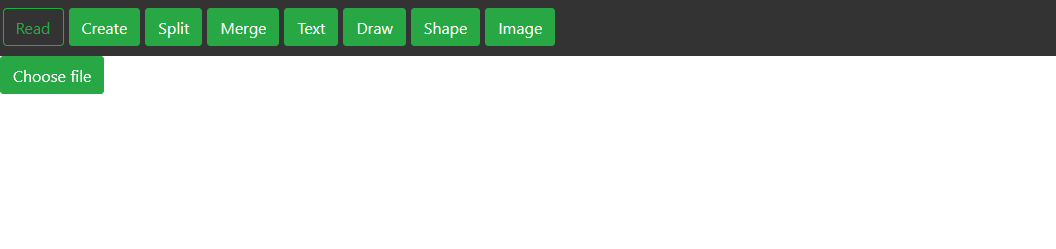
\includegraphics[width=1\textwidth]{"images/startseite.png"}
	\caption{Startseite der PDF Web App}
	\label{fig:start}
\end{figure}

Bei fast allen Modulen gibt es Möglichkeiten Benutzereingaben zu machen. Die Benutzereingaben sind so umgesetzt, dass sie bei ungültigem Input automatische korrigiert werden oder die darauf bezogene Operation nicht ausgeführt wird. Gibt man in ein input field, wo eine Zahl erwartet wird, einen String ein, so wird dessen Funktion nicht angewendet. Liegt eine Benutzereingabe als Zahl unter oder über dem minimalen oder maximalen Schwellenwert des Eingabefeldes, so wird die Eingabe mit dem niedrigsten oder obersten Wert substituiert. Manche Eingabefelder erwarten Integers, anstatt Floats, z.B. das input field für die Seitenzahl. In diesem Fall wird die Nachkommastelle automatisch von der Benutzereingabe entfernt. Haben sich beim Benutzer ein oder mehrere Leerzeichen in die Eingabe eingeschlichen, so werden diese Leerzeichen von der Anwendung automatisiert erkannt und entfernt. Falls eine andere Dateiart als .pdf, unabhängig vom Modul der App, geöffnet wurde, erscheint die Fehlermeldung in Screenshot \ref{fig:errorfile}. Auch beim Versuch eine verschlüsselte PDF-Datei zu öffnen, wird eine in Screenshot \ref{fig:errorcrypt} dargestellte Fehlermeldung angezeigt.

\begin{figure}[!htbp]
	\centering
	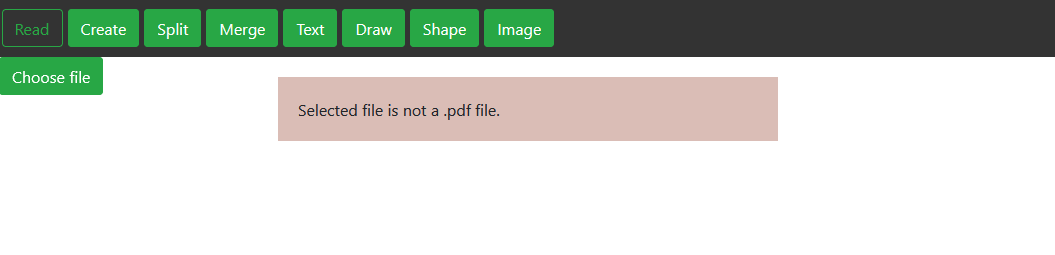
\includegraphics[width=1\textwidth]{"images/errorfile.png"}
	\caption{Fehlermeldung bei einer nicht-PDF-Datei}
	\label{fig:errorfile}
\end{figure}

\begin{figure}[!htbp]
	\centering
	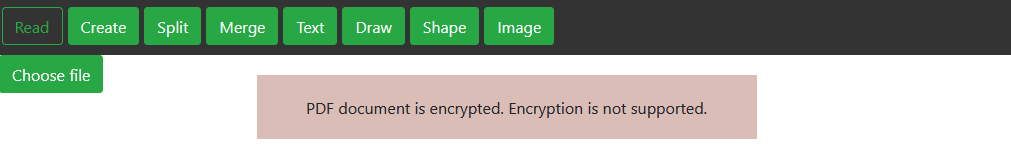
\includegraphics[width=1\textwidth]{"images/errorcrypt.png"}
	\caption{Fehlermeldung bei einem verschlüsselten PDF}
	\label{fig:errorcrypt}
\end{figure}

\begin{figure}[!htbp]
	\centering
	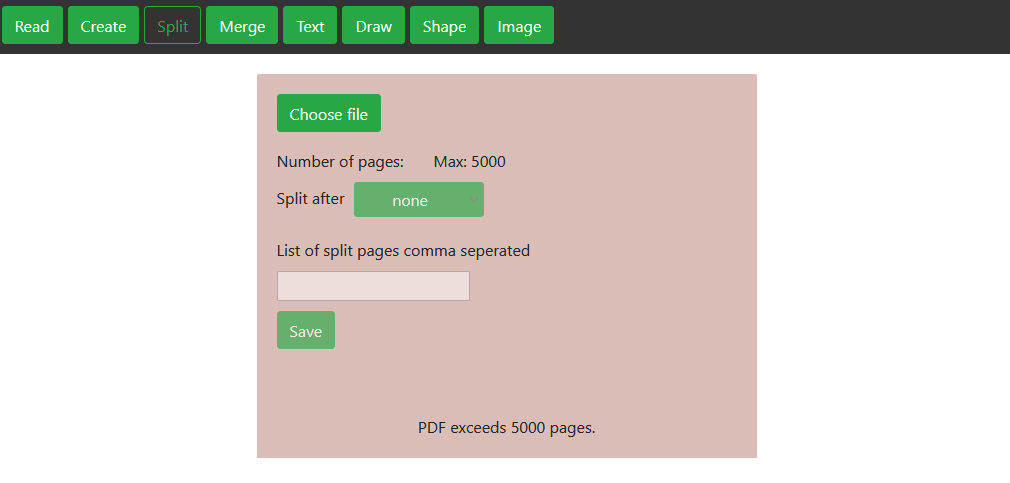
\includegraphics[width=1\textwidth]{"images/errorpages.png"}
	\caption{Fehlermeldung bei einem Input- oder Output-PDF mit mehr als 5000 Seiten}
	\label{fig:errorpages}
\end{figure}

Alle Module unterstützen Input- und Output-PDFs von maximal 5000 Seiten. Falls ein PDF mit mehr als 5000 Seiten geöffnet wird, erscheint eine entsprechende Fehlermeldung. Sie erscheint sogar im Merger, wenn man versucht ein PDF zu mergen, welches über 5000 Seiten hätte, was Screenshot \ref{fig:errorpages} visualisiert. Bei diesen gezeigten Fehlermeldungen kann man erneut den Dateibrowser im jeweiligen Modul öffnen und eine passende PDF-Datei auswählen oder einen anderen Hauptmenüpunkt wählen, damit die Fehlermeldung verschwindet. \\
Ist ein Modul der PDF Web App geöffnet, so wird der entsprechende Hauptmenübutton durch einen dunkelgrauen Hintergrund mit grüner Schrift symbolisiert. Initial ist der Reader ausgewählt. Der Button Create führt zum Creator für leere PDFs, Split zum Splitter für das Seiten Zerteilen, Merge zum Merger für das Zusammenfügen von PDF-Dateien, Text zum Writer für Textbearbeitung, Draw zum Drawer fürs Zeichnen, Shape zum Shaper zur Geometrieerstellung und Image zum Imager zur Bildbearbeitung. Befindet man sich im Reader, Merger, Splitter oder Creator und klickt dann auf ein Editormodul, so wird standardmäßig der Writer ausgewählt. Man muss dann nochmals auf ein anderes Editormodul klicken, um es auszuwählen. Jedes Modul der PDF Web App hat einen grünen Save-Button, mit dem der Benutzer das editierte PDF als ZIP-Archiv downloaden kann. Es wird im Downloads-Ordner im lokalen Dateisystem abgelegt. Bewegt man die Maus über den Save-Button erscheint eine schwarze Dialogbox, in der man einen benutzerdefinierten Dateinamen vergeben kann. Hat man einen benutzerdefinierten Dateinamen eingegeben, so erhält das Output-PDF und der ZIP-Ordner diesen Namen, ansonsten wird ein default Name verwendet, der aus dem Ursprungsdateinamen und einem Suffix besteht. Der Screenshot \ref{fig:save} bildet die Dialogbox zur Vergabe des Dateinamens ab. 

\begin{figure}[!htbp]
	\centering
	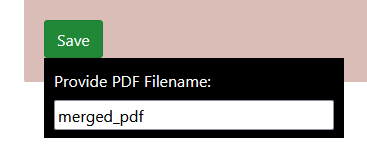
\includegraphics[width=0.6\textwidth]{"images/save.png"}
	\caption{Dateibenennungsdialog des Save-Buttons der PDF Web App}
	\label{fig:save}
\end{figure}

Bei Read, Text, Draw, Shape und Image erscheint zunächst der Choose file-Button, damit man im Dateisystem ein PDF-Dokument zum Lesen oder Bearbeiten auswählen kann. Klickt man auf Choose file wird der Dateibrowser geöffnet und man kann ein einzelnes PDF zum Öffnen auswählen. Ein geöffnetes Dokument passt seine Zoomgröße automatisch an das Browserfenster an, falls es bei 100 \% über das Browserfenster hinausragen würde, sodass es fast formatfüllend mit etwas Abstand zum Rand in den Viewport des Browserfensters passt. 

\subsection{Bedienung des Readers}
Der Reader mit geöffneter PDF-Datei präsentiert sich in Screenshot \ref{fig:reader}.

\begin{figure}[!htbp]
	\centering
	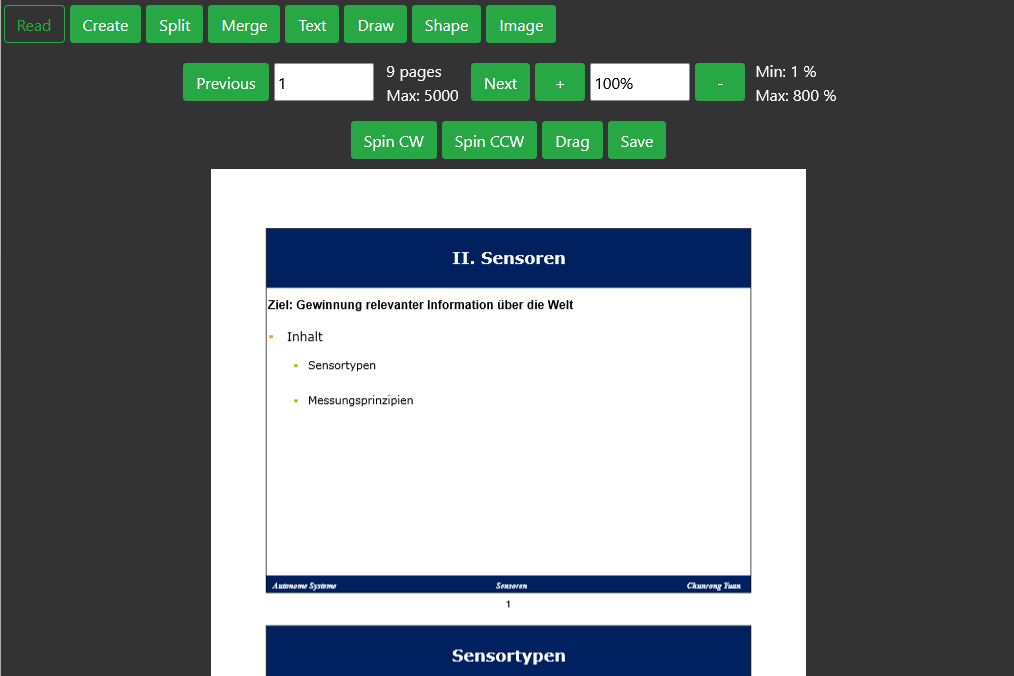
\includegraphics[width=1\textwidth]{"images/reader.png"}
	\caption{Geöffnetes PDF im Reader der PDF Web App}
	\label{fig:reader}
\end{figure}

Hat der Anwender eine PDF-Datei im Reader geöffnet, so entdeckt er 2 dunkelgraue Leisten mit Funktionsbuttons. Mittels Previous und Next kann der Benutzer zur vorherigen bzw. nächsten Seite blättern. Zwischen diesen Buttons informiert das pageCounter input field über die aktuelle Seite im Viewport und rechts daneben ist die Anzahl an Seiten im Dokument zu sehen. Im pageCounter input field kann man eine Seitenzahl des Dokuments eingeben, mit Enter bestätigen und der Reader springt direkt zu dieser Zielseite. Alternativ kann man mit dem Scrollbar am linken Browserfensterrand oder dem Scrollrad der Maus durch die Seiten scrollen. Mittels der Buttons Plus und Minus kann man in 20 \%-Schritten rein- bzw. rauszoomen. Der aktuelle Zoomwert in Prozent wird im input field dazwischen signalisiert. Der Anwender kann den Zoomwert auch auf einen gewünschten Wert mit oder ohne Prozentzeichen setzen und Enter drücken, damit der Zoomwert angewendet wird. Wird kein Prozentzeichen über die Tastatur eingegeben, sondern nur der Wert, so wird ein Prozentzeichen von der Anwendung hinzugefügt. Dabei werden nur ganze Zahlen ohne Nachkommastellen berücksichtigt. Außerdem wird der minimale und maximale Zoomwert in Prozent angezeigt. Spin CW und Spin CCW dreht die aktuelle Seite, die im pageCounter steht, um 90 Grad-Intervalle im Uhrzeigersinn (clockwise) und gegen den Uhrzeigersinn (counterclockwise). Durch den Button Drag kann man die aktuelle Seite im Viewport verschieben. Das ist beispielsweise nützlich, wenn man an das PDF besonders nah rangezoomt hat und die Seite nur teilweise sehen kann, weil man einen kleinen Laptopbildschirm besitzt. Dabei klickt man zuerst auf Drag, hält die Maustaste auf der aktuellen Seite gedrückt und bewegt sie in die gewünschte Richtung. Dabei verschiebt sich nicht nur die aktuelle Seite, sondern alle Seiten und der Mauscursor wechselt das Aussehen zu einem weißen Kreuz mit Pfeilen an den Enden.

\subsection{Bedienung des Creators}
Der Creator ist mittels des Create Buttons im Hauptmenü aufrufbar. Im Screenshot \ref{fig:creator} ist die GUI vom Creator dargestellt. 

\begin{figure}[!htbp]
	\centering
	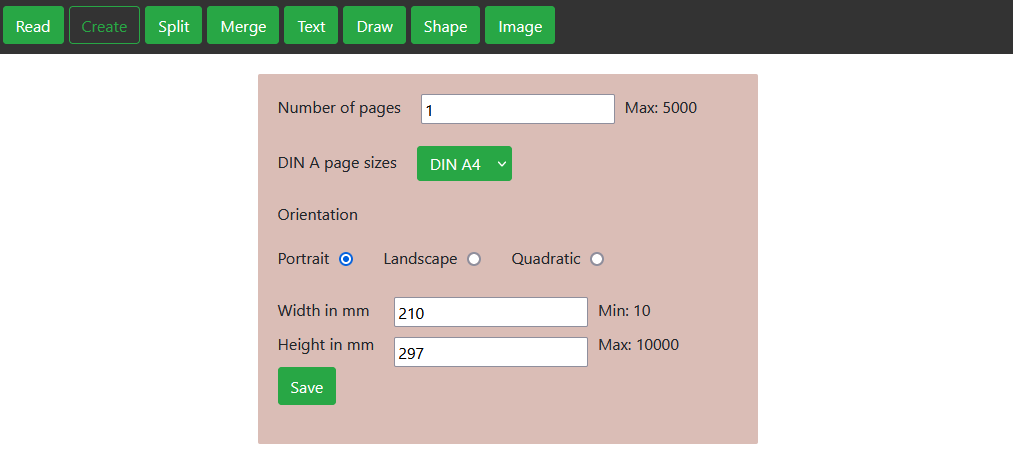
\includegraphics[width=1\textwidth]{"images/creator.png"}
	\caption{Creator GUI der PDF Web App}
	\label{fig:creator}
\end{figure}

\begin{figure}[!htbp]
	\centering
	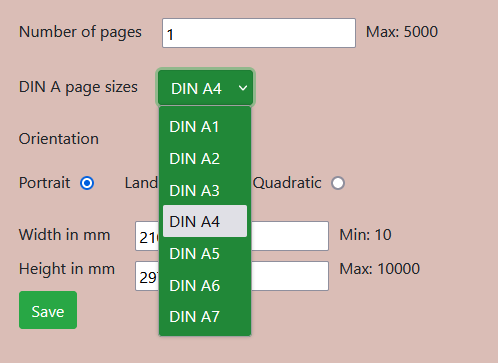
\includegraphics[width=0.7\textwidth]{"images/creator-sel.png"}
	\caption{Creator selection menu der PDF Web App}
	\label{fig:creator-sel}
\end{figure}

Man gibt eine Anzahl an gewünschten Seiten des leeren PDFs ein, sowie die Breite und Höhe in mm. Wahlweise kann man das grüne selection menu benutzen, um ein DIN A-Preset zu verwenden, was der Screenshot \ref{fig:creator-sel} darstellt. Mittels der Schnellauswahl kann man die Orientierung bestimmten: Portrait, Landscape oder Quadratisch. Minimale und maximale Werte für die Anzahl an Seiten und die Breite und Höhe sind ebenfalls abgebildet. 


\subsection{Bedienung des Splitters}
Zum Splitter kann man mit dem Split Button gelangen, dessen GUI vom Screenshot \ref{fig:splitter} gezeigt wird.

\begin{figure}[!htbp]
	\centering
	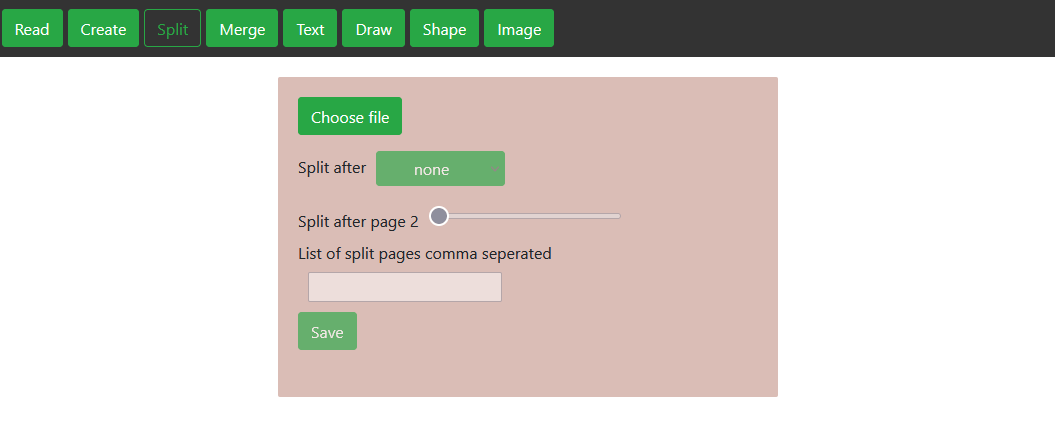
\includegraphics[width=1\textwidth]{"images/splitter.png"}
	\caption{Splitter GUI der PDF Web App}
	\label{fig:splitter}
\end{figure}

\begin{figure}[!htbp]
	\centering
	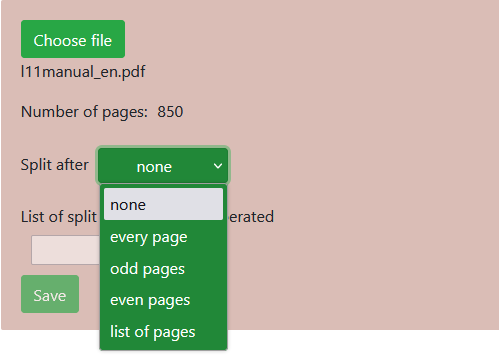
\includegraphics[width=0.7\textwidth]{"images/splitter2.png"}
	\caption{Splitter selection menu der PDF Web App}
	\label{fig:splitter2}
\end{figure}

Hat man eine Datei ausgewählt, so wird der Dateiname und die Anzahl an Seiten des Dokuments angezeigt. Durch erneutes Klicken des Choose file-Buttons öffnet sich abermals der Dateidialog und man kann ein anderes PDF auswählen. Dabei ersetzt das neue PDF das vorherige, denn man kann nicht mehrere PDF-Dateien gleichzeitig splitten. Im selection menu kann man zwischen Zerteilen nach ever page, odd pages, even pages und list of pages wählen, was in Abbildung \ref{fig:splitter2} dargestellt ist. Selektiert man list of pages, so kann man die einzelnen mit Komma separierten Seitennummern oder auch nur eine einzelne Seitennummern eintippen. Die Seitenzahlen müssen nicht in aufsteigender Reihenfolge angegeben werden. Bei ungültigen Eingaben wird das input field für die Seitenliste automatisch gelöscht. 

\subsection{Bedienung des Mergers}
Der Merger ist mit dem Hauptmenüpunkt Merge zu öffnen. Abbildung \ref{fig:merger} zeigt die Startseite des Mergers. 

\begin{figure}[!htbp]
	\centering
	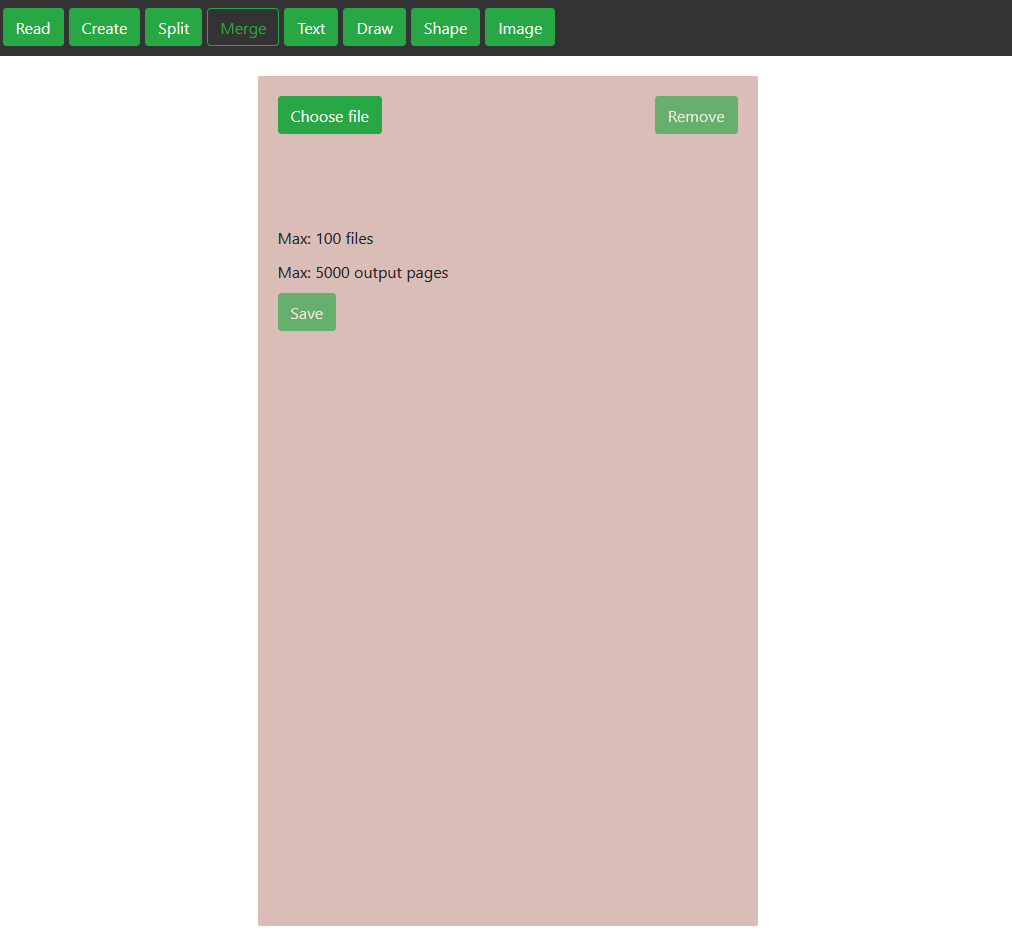
\includegraphics[width=1\textwidth]{"images/merger.png"}
	\caption{Merger Startseite der PDF Web App}
	\label{fig:merger}
\end{figure}

Hier kann man nacheinander mehrere Dateien mittels Choose file öffnen und sie erscheinen, je nach Auswahlreihenfolge, untereinander in einer scrollbaren Liste, wobei die zuerst ausgewählte Datei am Anfang der Liste steht. Es können maximal 100 Dateien der Liste hinzugefügt werden. In der Liste kann man dann eine Quelldatei mit gedrückter Maustaste zu einer Zieldatei in der Liste ziehen. Lässt man die Maustaste los, so wird die mit der Maus bewegte Datei in diese Listenposition eingefügt. Man kann außerdem eine Datei in der Liste selektieren und mittels des Remove-Buttons wieder aus der Liste entfernen. Eine selektierte Datei wird durch einen schwarzen Hintergrund, was der Screenshot \ref{fig:mergelist} verdeutlicht, symbolisiert.

\begin{figure}[!htbp]
	\centering
	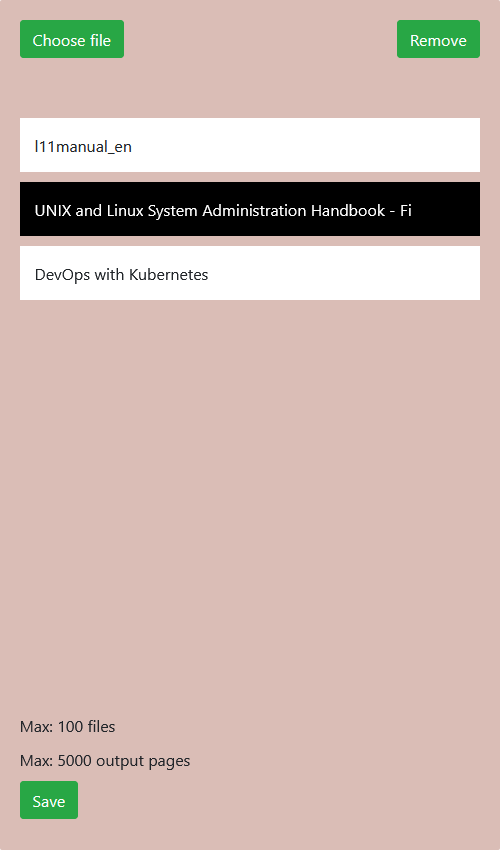
\includegraphics[width=0.7\textwidth]{"images/mergelist.png"}
	\caption{Merger Dateiliste der PDF Web App mit selektierter Datei}
	\label{fig:mergelist}
\end{figure}

Der Benutzer kann zu jeder Zeit erneut den Dateibrowser bedienen, unabhängig davon, ob die Dateiliste bereits modifiziert wurde und der Save-Button mergt alle PDF-Dateien in der gegenwärtigen Liste mit der obersten Datei zuerst und der letzten am Schluss des Output-PDFs.

\subsection{Bedienung des Editors}
Der Editor ist über den Text-, Draw-, Shape- oder Image-Button erreichbar. Ebenso wie im Reader erscheint zuerst ein Button Choose file. Je nachdem ob nach erstmaligem Öffnen einer PDF-Datei auf Text, Draw, Shape oder Image geklickt wurde, wird als erstes der Writer-, Drawer-, Shaper- oder Imager-Bearbeitungsmodus geöffnet. Ist eine Datei geöffnet, so ist der Reader, ohne die Operationen zum Seiten Drehen, Teil jedes Editormoduls. Alle input fields im Editor sind mit dem gültigen Wertebereich für Benutzereingaben als Information Min: Max: versehen. Der Editor samt dargestellter PDF-Datei besteht aus einem grauen, waagerechten Operations Bar, einem linken Layers Seitenmenü in Rosa und einem rechten grünen Tools Seitenmenü. Mit dem ganz linken, grünen Button Layers im Operations Bar kann das Layers Seitenmenü aus- und eingeblendet werden. Daneben zeigt oder verbirgt der Button Tools das Tools Seitenmenü. Standardmäßig sind Layers und Tools ausgeklappt. Beim Öffnen einer PDF-Datei, wird eine Infobox, die über den Fortschritt der gerenderten PDF-Seiten informiert, angezeigt. Ebenso wird eine Infobox angezeigt, die Auskunft darüber gibt, dass gerade der Speicherprozess in Gange ist. Hat man Text, Drawings, Shapes oder Images hinzugefügt und klickt auf Save, so wird das PDF zuerst auf 500 \% gezoomt, damit die Elemente als Bilder in hochwertiger Qualität eingebettet werden können. Am Ende des Speichervorgangs wird wieder auf den aktuellen Zoomwert des Benutzers zurück gezoomt. Diese beiden Infoboxen, die in Screenshot \ref{fig:render-info} und \ref{fig:save-info} abgebildet sind, sind auch im Reader vorhanden. Die einzelnen Speicherschritte werden in der Webkonsole der Web Developer Tools des Browsers ausgegeben, was in Bild \ref{fig:save-progress-steps} zu sehen ist.

\begin{figure}[!htbp]
	\centering
	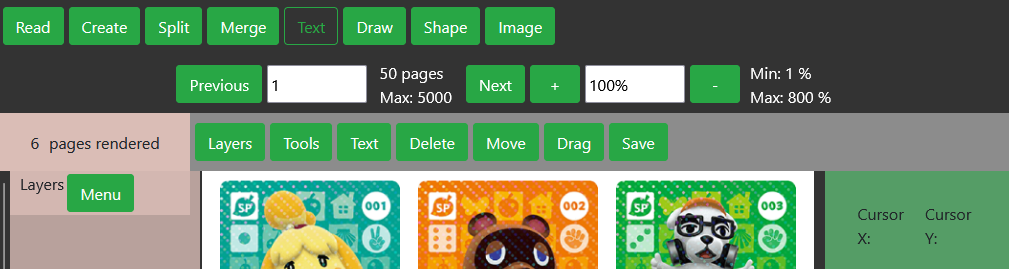
\includegraphics[width=1\textwidth]{"images/render-info.png"}
	\caption{Infobox über den Renderfortschritt der PDF Web App}
	\label{fig:render-info}
\end{figure}

\begin{figure}[!htbp]
	\centering
	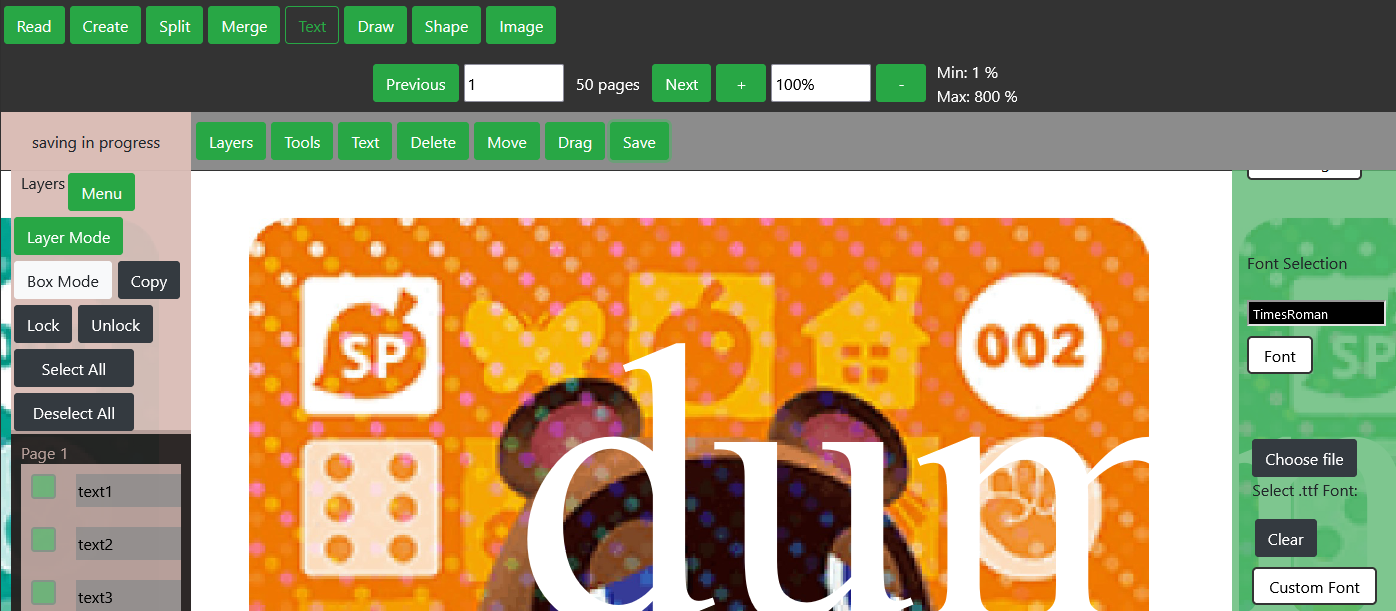
\includegraphics[width=1\textwidth]{"images/save-info.png"}
	\caption{Infobox über den Speicherprozess der PDF Web App}
	\label{fig:save-info}
\end{figure}

\begin{figure}[!htbp]
	\centering
	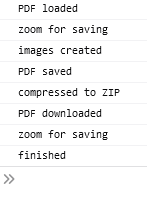
\includegraphics[width=0.4\textwidth]{"images/save-progress-steps.png"}
	\caption{Speicherschritte der PDF Web App in der Webkonsole beim Speichern von Elementen}
	\label{fig:save-progress-steps}
\end{figure}

\subsubsection{Textbearbeitung}
Hat man den Writer aufgerufen, so präsentiert sich einem der Texteditor in den folgenden Abbildungen \ref{fig:texteditor} und \ref{fig:texteditor2}.

\begin{figure}[!htbp]
	\centering
	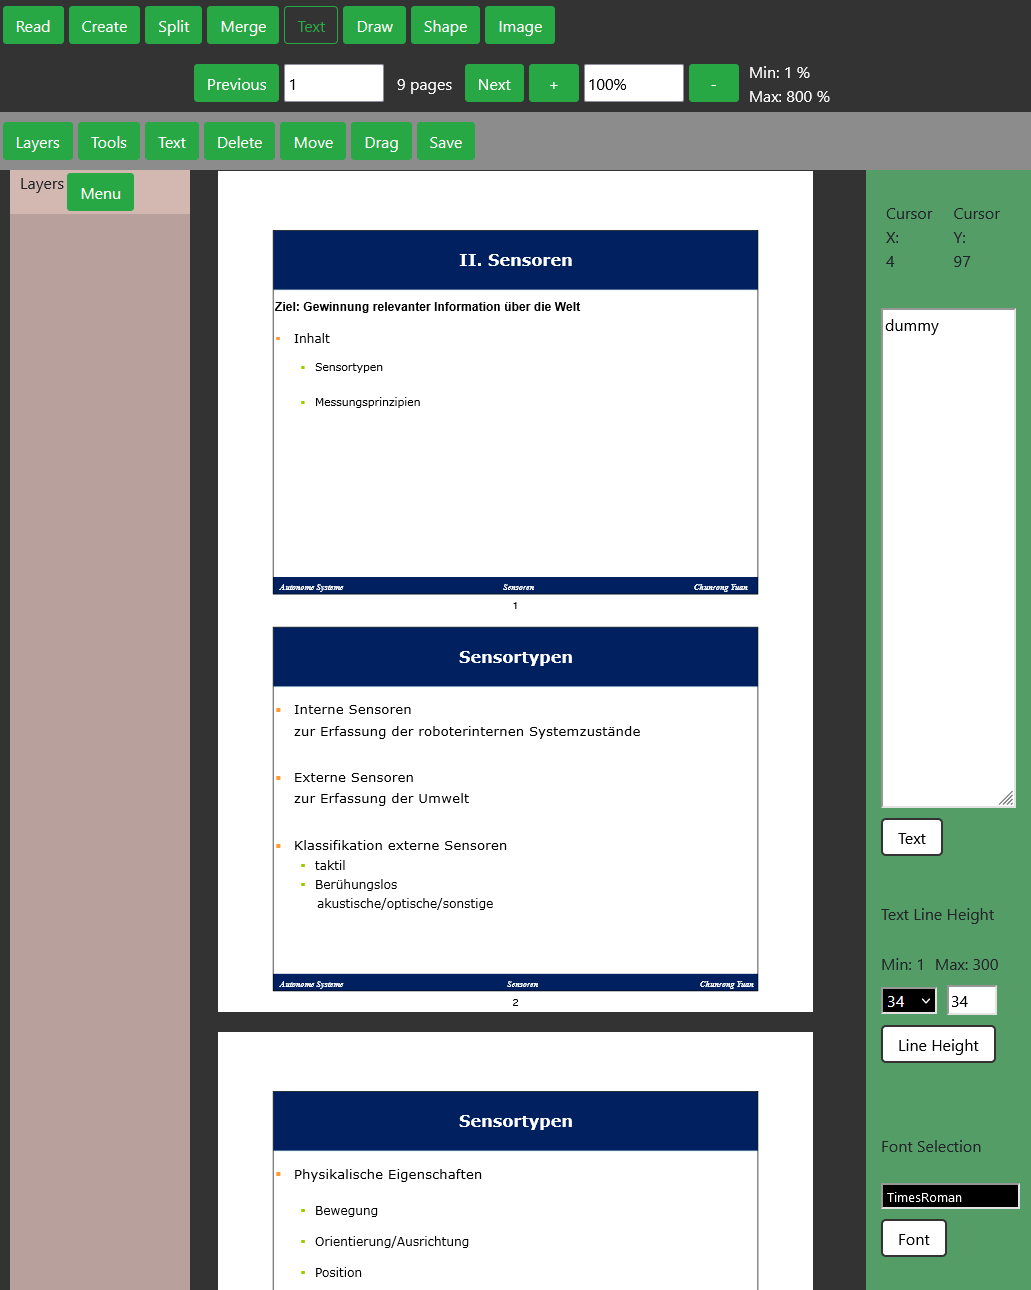
\includegraphics[width=1\textwidth]{"images/texteditor.png"}
	\caption{Startseite des Writers der PDF Web App}
	\label{fig:texteditor}
\end{figure}

\begin{figure}[!htbp]
	\centering
	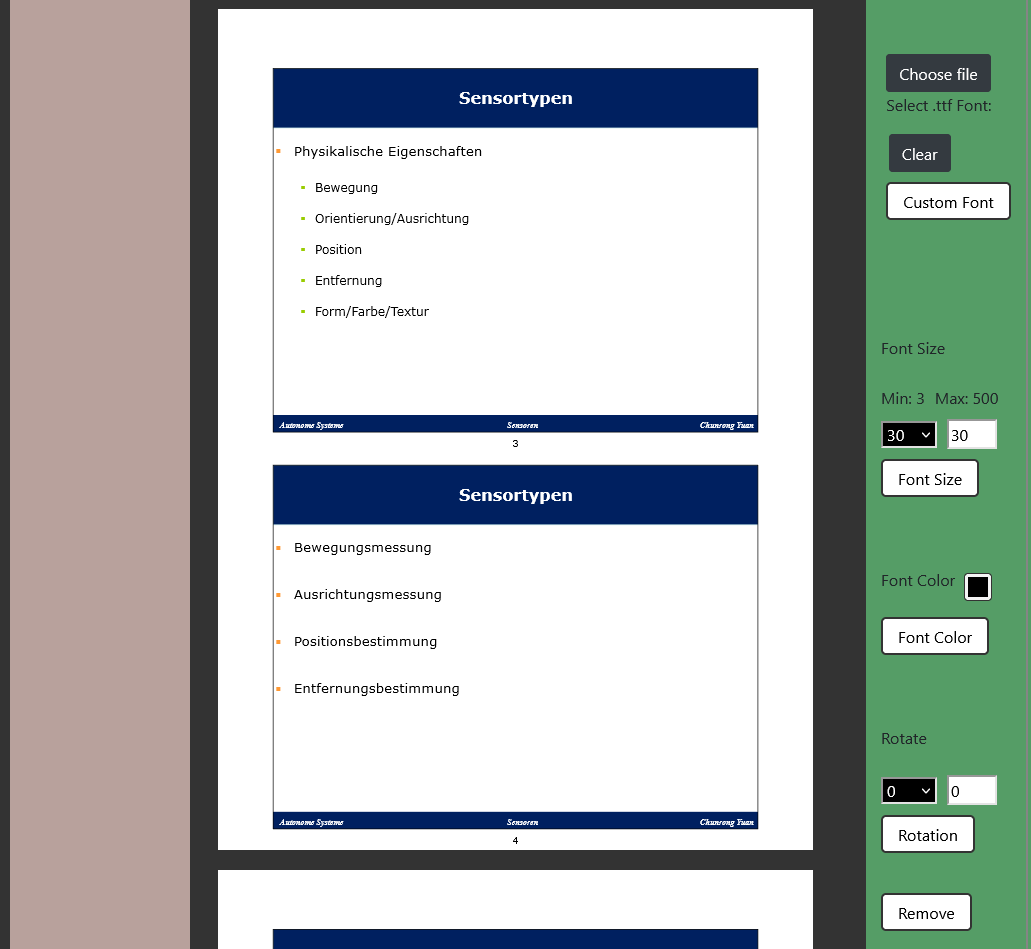
\includegraphics[width=1\textwidth]{"images/texteditor2.png"}
	\caption{Mehr Tools der Startseite des Writers der PDF Web App}
	\label{fig:texteditor2}
\end{figure}

Mit dem Button Text im Operations Bar und nachfolgendem Klick auf das geöffnete Dokument, wird der Platzhaltertext dummy hinzugefügt. Unter dem Text erscheint eine dunkelrote controlBox, auf die man alle Operationen im Operations Bar und in Tools im Box Mode anwenden kann. Ich werde zunächst alle Operationen im Box Mode beschreiben und später auf den Layer Mode eingehen. Der Box Mode ist standardmäßig eingestellt. Operationen können durch die grünen Buttons zum Erstellen neuer Elemente, Delete und Move im Operations Bar und allen weißen Buttons in Tools getriggert werden. Hat man eine Operation getriggert, so befindet man sich im Modus dieser Operation im Box Mode. Darauffolgend können alle, im Dokument verfügbaren controBoxes angeklickt werden, um die Operation auf das betreffende Element auszuführen. Alle Operationen in Tools beziehen sich jeweils auf das Element des aktuellen Editormoduls und sind nur auf diesem anwendbar. Versucht man eine Operation eines Editormoduls auf ein Element eines anderes Editormoduls anzuwenden, wird die Operation nicht ausgeführt. In der Praxis des Box Modes kann man mehrere Texte, ohne erneut den grünen Text Button drücken zu müssen, dem PDF-Dokument hinzufügen. Für jedes neu hinzugefügte Editorelement wird eine Layer, mit einem elementspezifischen Standardnamen erstellt, die in Layers erscheint. Die obere linke Ecke der quadratischen controlBox von sämtlichen Editorelementen wird an der Stelle platziert, an der man mit der Maus auf die Seite geklickt hat. Alle controlBoxes werden nicht im  Output-PDF gespeichert, denn sie dienen lediglich der Steuerung von Editorelementen, um Operationen im Box Mode anwenden zu können. Mit dem Delete-Button und nachfolgendem Klick in eine oder mehrere controlBoxes im Box Mode, können Texte wieder gelöscht werden. Move verschiebt einzelne Texte durch eine mit der Maus gedrückten und zur Zielposition bewegten controlBox. Sobald die Maus losgelassen wird, nachdem die controlBox verschoben wurde, springt der Text an die Zielposition auf der Seite. Dabei ist wichtig zu beachten, dass man die controlBox langsam verschiebt, denn der Mauszeiger muss innerhalb der controlBox bleiben. Delete und Move kommen in allen Editormodulen vor und funktionieren immer gleich. Ganz oben in Tools werden dem Betrachter die x- und y-Koordinaten des Mauscursors auf der PDF-Seite angezeigt, während die Maus über eine Seite bewegt wird. Diese Mauscursorkoordinaten sind in jedem Editormodul präsent. Textelemente lassen sich in der textarea editieren. Zeilenumbrüche werden berücksichtig. Nachdem der dummy Text in der textarea überschrieben wurde, ein Klick auf den weißen Text-Button erfolgte und die Operation auf eine controlBox angewendet wurde, substituiert sich der Platzhaltertext mit dem aktuellen Text in der textarea. Die textarea kann in vertikaler Höhe expandiert werden. In allen Editormodulen von Tools werden alle Operationen exakt gleich ausgeführt: Man tätigt seine Einstellung, drückt mit der linken Maustaste auf den weißen Button für die jeweilige Operation und klickt daraufhin auf eine oder mehrere controlBoxes von Elementen. Unterhalb der Texteditierungsoperation kann der Zeilenabstand einstellt werden. Entweder verwendet man das selection menu mit voreingestellten Werten oder man gibt einen gewünschten Wert manuell in das input field ein. Neu hinzugefügte Elemente sind standardmäßig vorkonfiguriert. Alle Eingabefelder sämtlicher Editormodule zeigen dessen Standardwerte an. Bei jeder selection menu und input field Kombination ist maßgeblich, welche Schaltfläche zuletzt betätigt wurde. Einen benutzerdefinierten Font als .ttf oder .otf Datei kann man durch den dunkelgrauen Choose file-Button vom Dateisystem auswählen und wird in einer Liste abgebildet. Der zuletzt geöffnete Font wird ausgewählt. Die Selektion des aktuellen Fonts wird durch einen Klick auf den radio button des Fontdateinamens aktiviert. Mittels Clear werden alle Fonts aus der Liste entfernt. Fontdateinamen werden nach 15 Zeichen in die nächste Zeile umgebrochen. Abbildung \ref{fig:custom-font} zeigt 2 geöffnete .ttf Schriftdateien in der Liste.

\begin{figure}[!htbp]
	\centering
	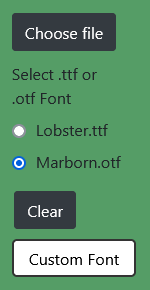
\includegraphics[width=0.2\textwidth]{"images/custom-font.png"}
	\caption{Benutzerdefinierte Fontliste im Texteditor der PDF Web App}
	\label{fig:custom-font}
\end{figure}

Die Fontgröße kann mittels selection menu und input field justiert werden. Bezüglich der Fontfarbe lässt sich ein Color Picker Menü mit Klick auf das initial schwarze Quadrat ausklappen. Es können Farbe und Transparenz eingestellt werden. Die Farbwerte stehen in den Formten RGBA, HSLA oder HEX zur Verfügung. Mit Klick auf die beiden kleinen senkrechten Pfeile im Color Picker wird das Format gewechselt. Das Fenster des Color Pickers für die Fontfarbe ist in Abbildung \ref{fig:fontcolor} dargestellt. 

\begin{figure}[!htbp]
	\centering
	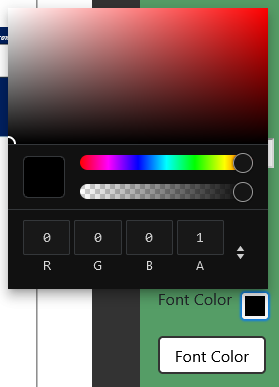
\includegraphics[width=0.5\textwidth]{"images/fontcolor.png"}
	\caption{Color picker für die Fontfarbe des Texteditors der PDF Web App}
	\label{fig:fontcolor}
\end{figure}

Als vorletzte Option kann der Text absolut gedreht werden. Durch den weißen Button Rotation und der entsprechenden Benutzerinteraktion durch selection Menu oder input field wird das Textelement rotiert. Absolute Rotation bedeutet, dass es eine feste Rotationsskala gibt, anhand der das Element rotiert wird. Bei einem Rotationswinkel von 0 Grad ein wird die Ausgangsrotation angewendet. Alle Editormodule arbeiten mit absoluter Rotation. Abschließend können alle Textelemente im Dokument mit dem Remove Button vollständig gelöscht werden. Ein neuer und modifizierter Text wird in Abbildung \ref{fig:text} demonstriert.

\begin{figure}[!htbp]
	\centering
	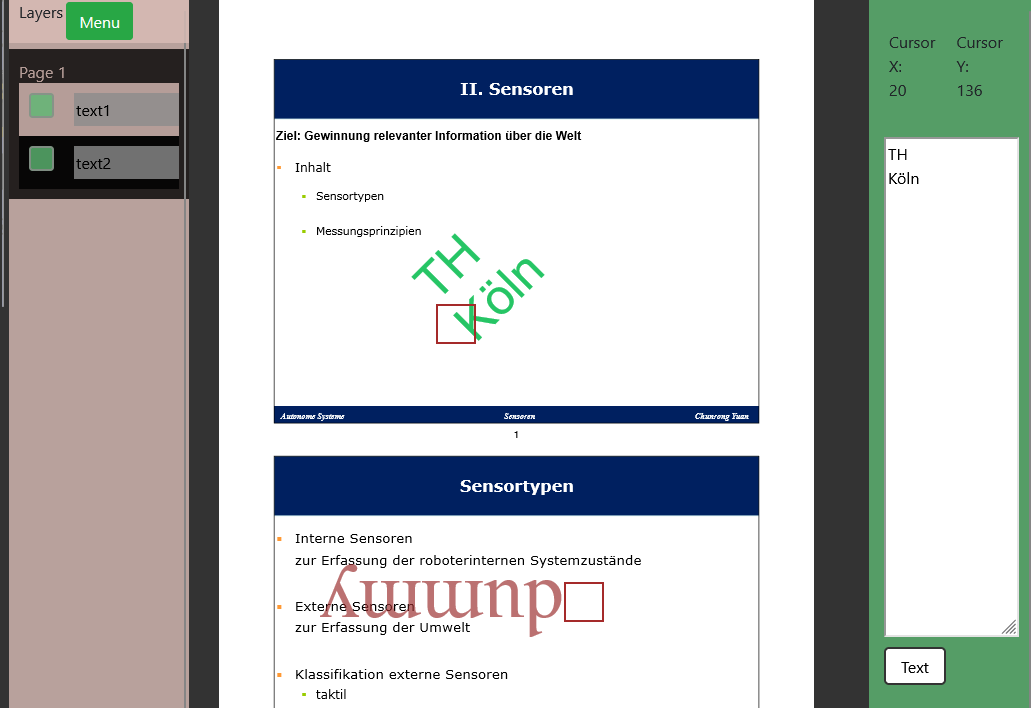
\includegraphics[width=1\textwidth]{"images/text.png"}
	\caption{Bearbeiteter Text im Writer der PDF Web App}
	\label{fig:text}
\end{figure}

\subsubsection{Drawings erstellen}
Der Drawer ist in Screenshot \ref{fig:drawer} abgebildet. 

\begin{figure}[!htbp]
	\centering
	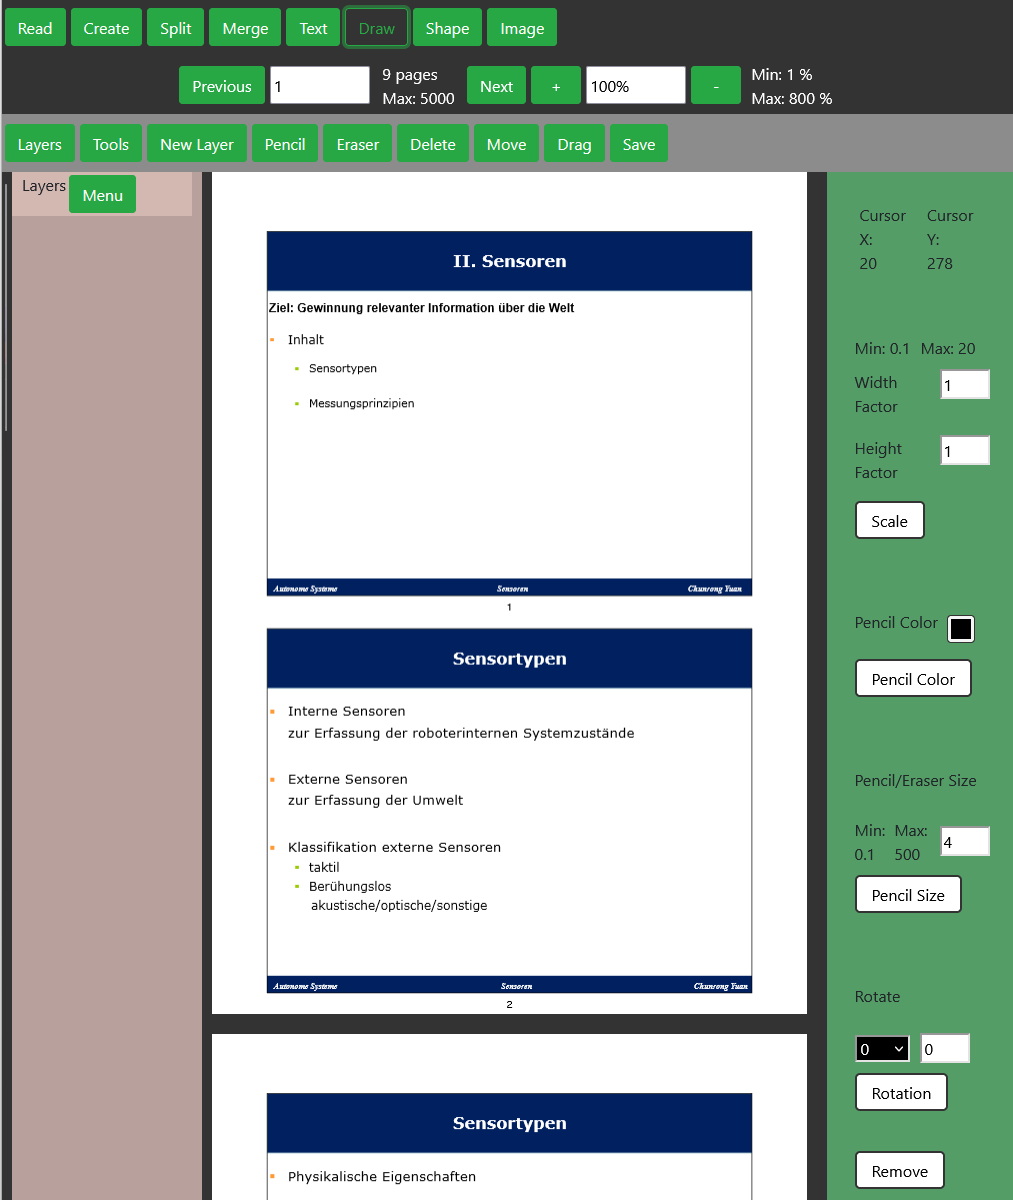
\includegraphics[width=1\textwidth]{"images/drawer.png"}
	\caption{Drawer der PDF Web App}
	\label{fig:drawer}
\end{figure}

Der Zeichenmodus wird mittels Pencil initiiert. Mit gedrückter Maustaste und gleichzeitigen Mausbewegungen erscheint eine Linie. Die Startstelle des Drawings wird durch eine magenta farbige controlBox markiert. Drawings lassen sich idealerweise mit einem Graphic Tablet erstellen. Für das erste Drawing der Seite wird von der Anwendung eine Layer zugewiesen. Mittels des New Layer-Buttons kann eine neue Layer kreiert werden. Falls keine Layer ausgewählt wurde, wird auf der zuletzt gezeichneten Layer der Seite gearbeitet. Generell wird auf der ausgewählten Layer gezeichnet. Der Radierermodus wird durch den Eraser-Button im Operations Bar aktiviert. Mit gedrückter Maustaste können Pixelbereiche des Drawings entfernt werden. Das Drawing zum Radieren wird durch die Auswahl der Layer bestimmt. Das Mauscursorsymbol der Zeichenoperation wird durch ein schwarzes, dünnes Kreuz signalisiert. Im Radierermodus alterniert das Mauscursorsymbol zu einem weißen, dicken Kreuz. Sobald eine Operation in Tools angewendet wird, wird der Zeichenmodus bzw. Radierermodus verlassen. In Tools kann ein Drawing relativ skaliert werden, indem ein Faktor eingegeben wird. Der Faktor kann auch ein Float sein und multipliziert sich immer mit der aktuellen Größe. Im nächsten Bereich definiert ein Color Picker die Stift- und Eraserfarbe inklusive der Deckkraft. Des Weiteren kann der Durchmesser des Stifts bzw. Radierers justiert werden. Ebenfalls können Drawings absolut rotiert werden. Wurde ein Drawing gedreht und auf der Layer weiter gezeichnet, so wird eine weitere Layer von der Anwendung angelegt. In der untersten Sektion von Tools entfernt Remove alle Drawings im Dokument. Teilweise transparente Drawings werden in Abbildung \ref{fig:drawing} dargestellt. 

\begin{figure}[!htbp]
	\centering
	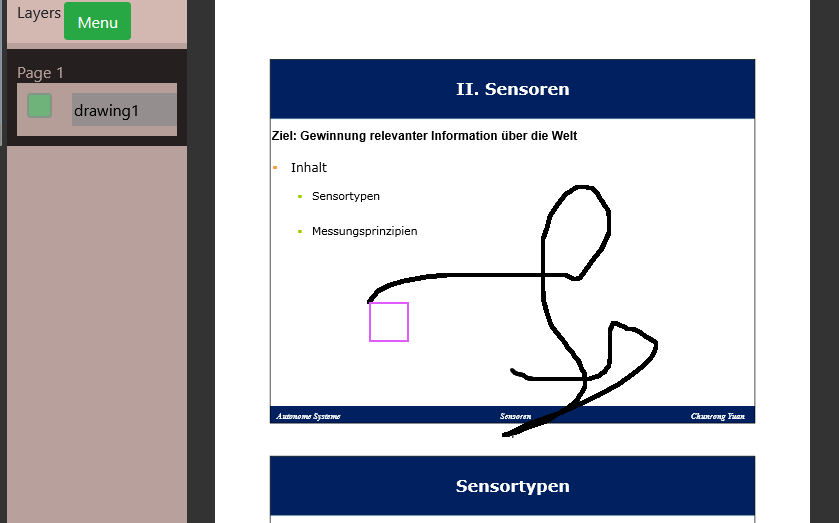
\includegraphics[width=1\textwidth]{"images/drawing.png"}
	\caption{Drawings im Drawer der PDF Web App}
	\label{fig:drawing}
\end{figure}


\subsubsection{Shapes hinzufügen}
Die Startseite des Shapers ist in den Screenshots \ref{fig:shaper} und \ref{fig:shaper2} abgebildet. 

\begin{figure}[!htbp]
	\centering
	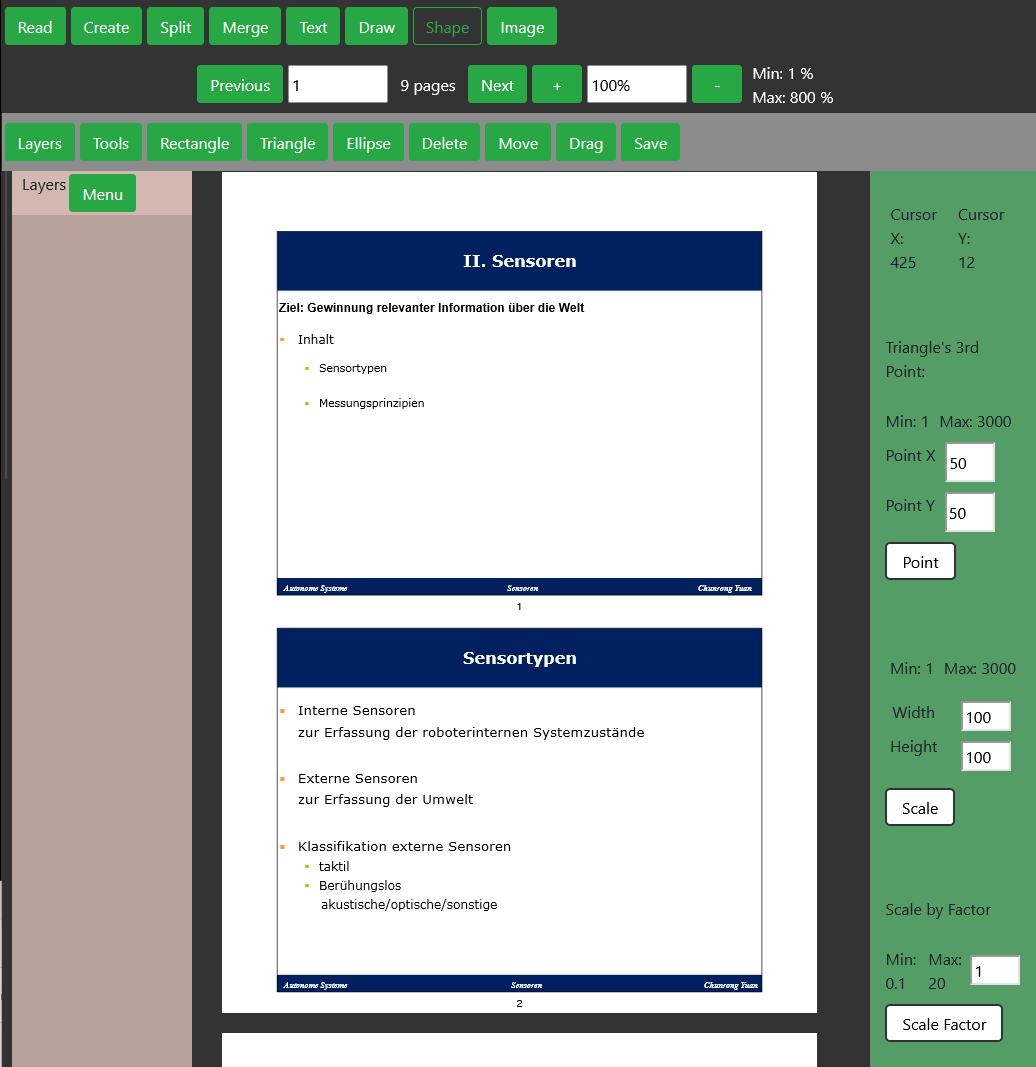
\includegraphics[width=1\textwidth]{"images/shaper.png"}
	\caption{Shaper der PDF Web App}
	\label{fig:shaper}
\end{figure}

\begin{figure}[!htbp]
	\centering
	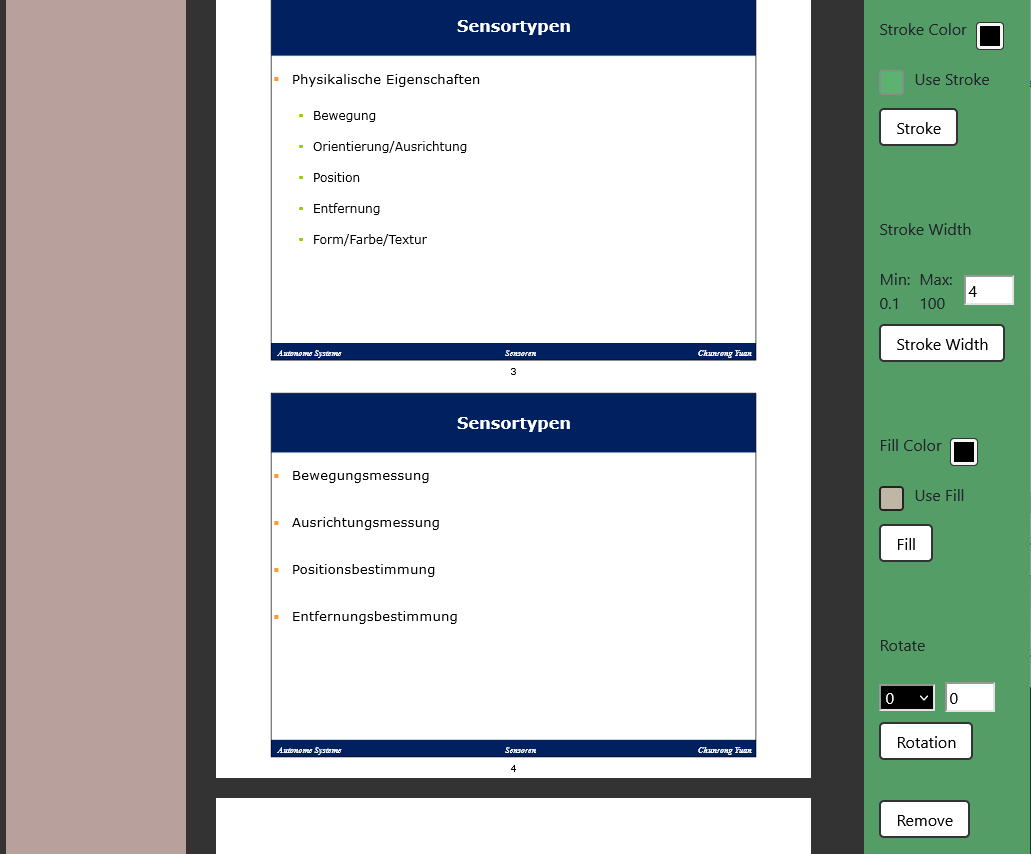
\includegraphics[width=1\textwidth]{"images/shaper2.png"}
	\caption{Mehr Tools des Shapers der PDF Web App}
	\label{fig:shaper2}
\end{figure}

Der Shapetyp kann durch die Buttons Rectangle für Rechteck, Triangle für Dreieck oder Ellipse und einem oder mehreren Klicks auf eine Seite bestimmt werden. Jedem Shape wird eine orange controlBox mehr oder weniger mittig hinzugefügt. In Tools des Shapers gibt es eine einzige Operation, die nur auf Dreiecke angewendet werden kann. Es handelt sich um die oberste Einstellung für die Breite und Höhe des dritten Punktes des Dreiecks (Triangle's Third Point). Mit dieser Operation kann der rechte Punkt der langen Spitze des default Dreiecks bearbeitet werden. Alle anderen Einstellmöglichkeiten können auf sämtlichen Shapeelementen Rectangle, Triangle und Ellipse arbeiten. Die Skalierung von Shapes bietet 2 Vorgehensweisen. Zum einen können Breite und Höhe unabhängig voneinander einstellt werden, was eine absolute Skalierung bedeutet. Zum anderen kann der proportionale, relative Skalierungsfaktor die Größe modulieren. Für die Umrandungslinien des Shapes kann auf der einen Seite die Farbe inklusive Deckkraft und auf der anderen Seite die Breite der Linie justiert werden. Die Strichfarbe muss mit der checkbox Use Stroke in Grün aktiviert sein. Bei Deaktivierung von Use Stroke schaltet sich automatisch die Use Fill checkbox ein und umgekehrt. Beide checkboxes können angehakt (Grün) sein, aber nicht beide zusammen abgehakt (Rosa). Use Fill muss Grün sein, um die Füllfarbe anzuwenden. Bei Strich- und Füllfarbe wird ein Color Picker verwendet. Alle Shapes können mit absoluter Rotation gedreht werden. Die controlBoxes werden durch die Rotation mitgedreht. Zuunterst entfernt der Remove-Button alle Shapes im Dokument. Der Screenshot \ref{fig:shaping} hebt mehrere bearbeitete Shapes hervor.

\begin{figure}[!htbp]
	\centering
	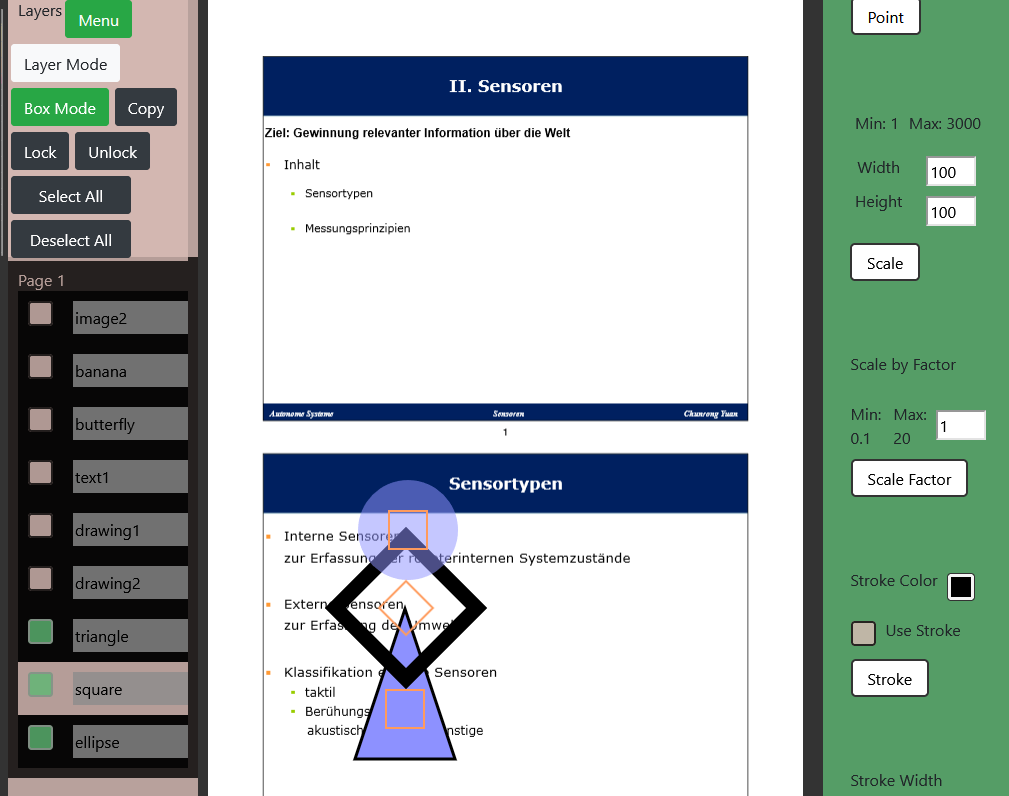
\includegraphics[width=1\textwidth]{"images/shaping.png"}
	\caption{Shapes im Shaper der PDF Web App}
	\label{fig:shaping}
\end{figure}


\subsubsection{Images einfügen}
Der Imager ist in Bild \ref{fig:images} dargestellt. 

\begin{figure}[!htbp]
	\centering
	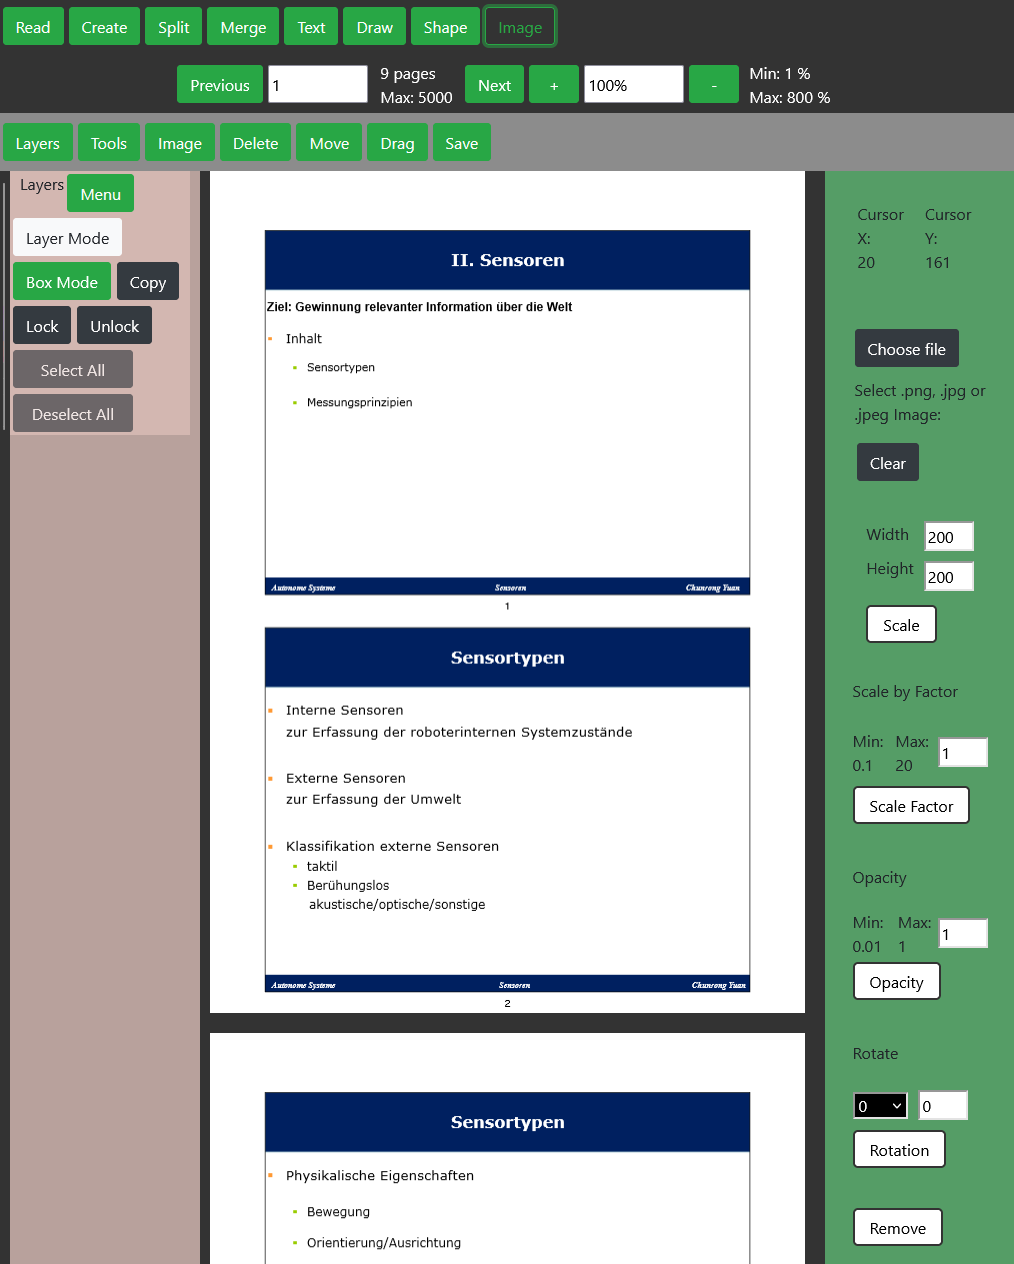
\includegraphics[width=1\textwidth]{"images/images.png"}
	\caption{Imager der PDF Web App}
	\label{fig:images}
\end{figure}

Um ein Image mit dem Image-Button im Operations Bar hinzuzufügen, muss zunächst ein Image mittels des dunkelgrauen Choose file-Buttons im Dateisystem ausgewählt werden. Dadurch erscheint der Imagename in der Liste unter Choose file. Mehrere Images lassen sich nacheinander mittels des Dateidialogs auswählen. Das zuletzt selektierte Image wird automatisch mit einem blauen radio button gekennzeichnet. Zusätzlich werden die Originaldimensionen des Images angezeigt, sobald das Image mittels des grünen Buttons Image im Operations Bar auf der Seite platziert wurde. Eine hellblaue controlBox erscheint bei der Imageplatzierung. Ein Image kann in Breite und Höhe absolut skaliert werden. Auf proportionale Art und Weise wird ein Image mit dem relativen Skalierungsfaktor verkleinert bzw. vergrößert. Unterhalb der Skalierungsoperationen kann die Deckkraft eines Images bestimmt werden. Ebenfalls lässt sich ein Image absolut rotieren. Zuletzt können alle Images im Dokument mit dem Remove-Button entfernt werden. Die Abbildung \ref{fig:imaging} zeigt den Imager in Aktion.

\begin{figure}[!htbp]
	\centering
	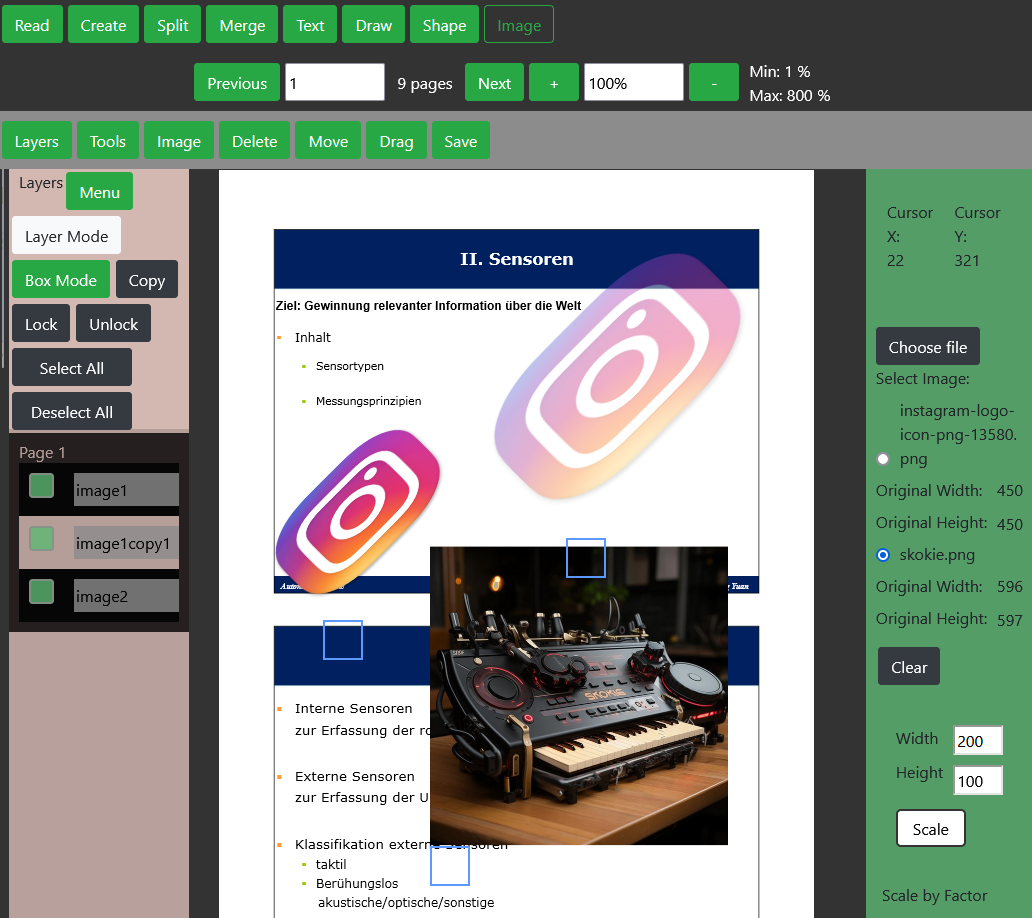
\includegraphics[width=1\textwidth]{"images/imaging.png"}
	\caption{Platzierte Images im Imager der PDF Web App}
	\label{fig:imaging}
\end{figure}

\subsubsection{Ebenensteuerung}
Das in Abbildung \ref{fig:ebenenmenu} gezeigte Layers Menu lässt sich mit einem Klick auf Menu in Layers hervorholen oder verbergen. Es ist möglich durch die Liste an hinzugefügten Layers zu scrollen.

\begin{figure}[!htbp]
	\centering
	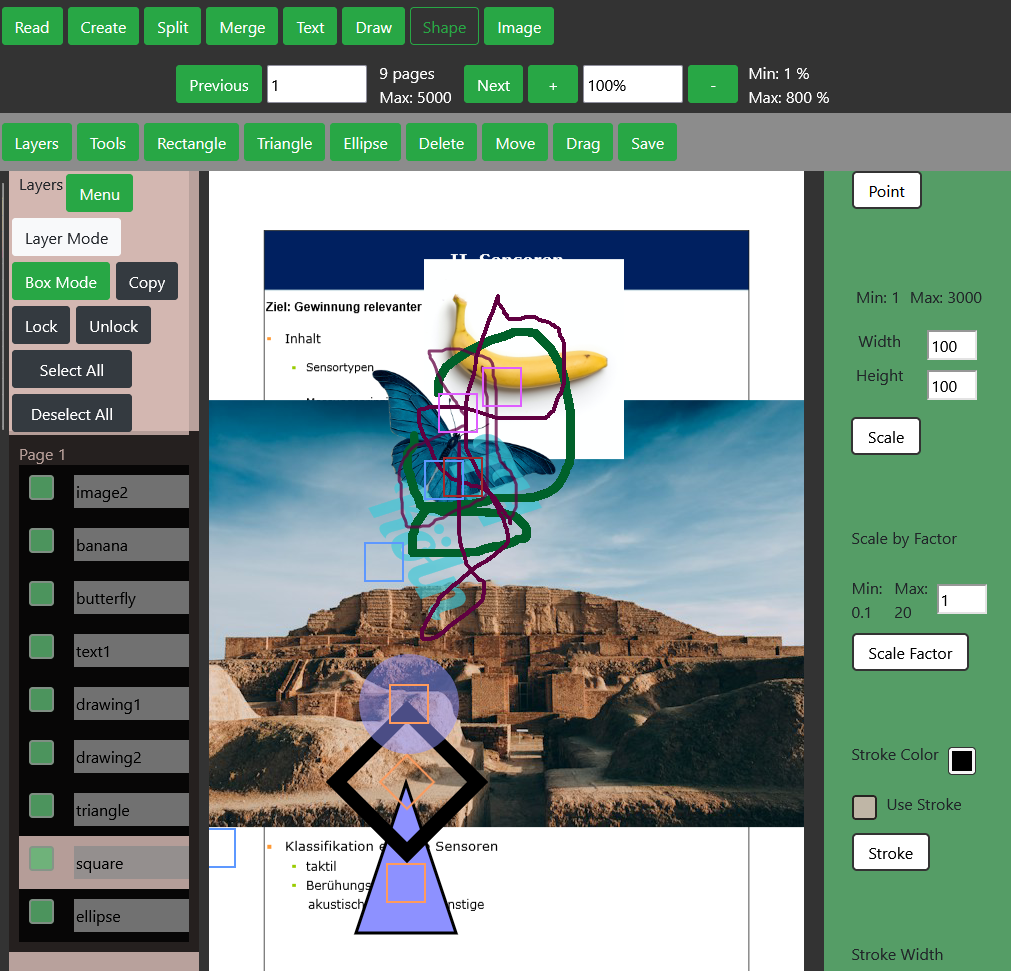
\includegraphics[width=1\textwidth]{"images/ebenenmenu.png"}
	\caption{Ausgeklapptes Layers Menu im Editor der PDF Web App}
	\label{fig:ebenenmenu}
\end{figure}

Standardmäßig sind die Schaltflächen eingeklappt. Fügt man ein Element, unabhängig vom Typ, einer PDF-Seite hinzu, wird für dieses Element eine Layer angelegt, die dann automatisch ausgewählt ist. Layers werden nach aufsteigenden Seitenzahlen gruppiert. Eine ausgewählte Layer ist rosa und eine abgewählte schwarz. Es können mehrere Layers ausgewählt werden. Wenn eine Layer angelegt wird, bekommt sie einen Standardnamen gesetzt, der durch den Elementtyp und einem nummerischen Index, beginnend mit 1, gekennzeichnet ist. Der Standardname kann durch Tastatureingabe im grauen input field auf der Layer überschrieben werden. Layers werden nach Seitenzahlen in einer schwarzen Box, die oberhalb mit der Seitenzahl gekennzeichnet ist, gruppiert. Im Layers Menu kann man zwischen Box Mode und Layer Mode wechseln. Ist der Modus Button grün, so ist der betreffende Modus eingeschaltet. Hingegen ist ein ausgeschalteter Modus mit einem weißen Button versehen. Man kann sich entweder im Box Mode, oder im Layer Mode befinden, aber nicht in beiden Modi gleichzeitig. Mit dem dunkelgrauen Copy-Button kann der Benutzer ausgewählte Layers kopieren. Folglich werden die beinhaltenden Elemente dubliziert. Wird eine Layer kopiert, so wird an den Layernamen copy und eine Nummerierung angehängt. Mit Lock und Unlock kann man Layers sperren bzw. entsperren. Eine locked Layer kann nicht verändert werden, d.h. keine Operationen können auf ihr beinhaltendes Element angewendet werden. Eine locked, unausgewählte Layer ist weiß und eine locked, ausgewählte ist rosa mit weißer Umrandung. 

\begin{figure}[!htbp]
	\centering
	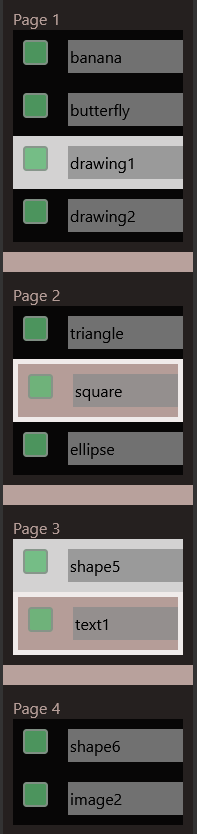
\includegraphics[width=0.3\textwidth]{"images/ebenen.png"}
	\caption{Teilweise locked Layers im Editor der PDF Web App}
	\label{fig:ebenen}
\end{figure}

Die dunkelgrauen Select All und Deselect All Buttons stellen Auswahlfilter dar. Bewegt man die Maus auf die Buttons klappt sich ein Selection Filter Menu auf, was im Bildausschnitt \ref{fig:filtermenu} gezeigt wird. 

\begin{figure}[!htbp]
	\centering
	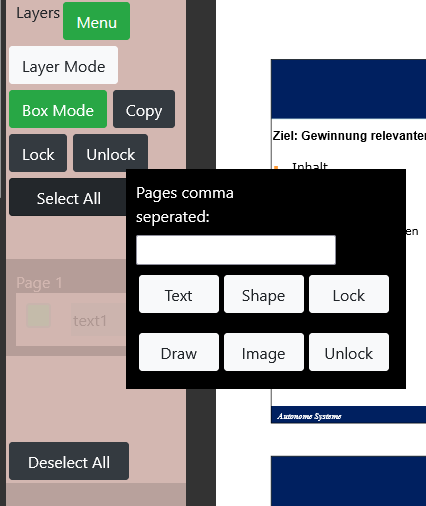
\includegraphics[width=0.6\textwidth]{"images/filtermenu.png"}
	\caption{Selection Filter Menu im Editor der PDF Web App}
	\label{fig:filtermenu}
\end{figure}

Bei Select All kann man mehrere Layers nach Seiten auswählen, nach Elementtyp und, ob sie locked oder unlocked sind, d.h. die Layers werden rosa markiert. Ist ein Selection Filter aktiviert, werden die Buttons im Selection Filter Menu grün. Bei weißen Buttons oder einer leeren Liste an Seiten ist kein Selection Filter aktiviert. Bei der Seitenliste muss man die Seiten durch Komma trennen und sie müssen nicht in aufsteigender Reihenfolge angegeben werden. Die Filter werden mit einem Klick auf Select All angewendet. Ist kein Filter aktiviert, was der Standardzustand ist, so werden alle Layers mit Klick auf Select All ausgewählt. Deselect All hat die gleiche Funktionalität, nur dass die Deselection Filter zum Auswahl aufheben angewendet werden, d.h. Layers werden auf Schwarz gesetzt. Ein Klick auf Deselect All ohne Filter wählt alle Layers im Dokument ab. Im Bildausschnitt \ref{fig:filtering.} ist ein Beispiel von Deselect All Filtern abgebildet. Laut des Beispiels würde die Auswahl auf allen unlocked Textelementen auf Seite 1 und 2 aufgehoben werden. 

\begin{figure}[!htbp]
	\centering
	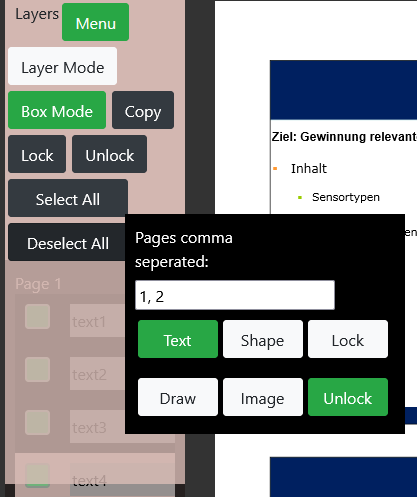
\includegraphics[width=0.6\textwidth]{"images/filtering.png"}
	\caption{Deselection Filter Menu mit aktivierten Filtern im Editor der PDF Web App}
	\label{fig:filtering}
\end{figure}

Sowohl bei Select All als auch bei Deselect All habe ich eine Benutzereingabenkontrolle beim der Seitenlistenfilter implementiert. Falls der Benutzer ungültige Eingaben gemacht hat, z.B. Seiten als Float oder Strings, so wird die Eingabe bei Auslösung des Filters gelöscht. Leerzeichen können zwischen gültigen Seitenzahlen verwendet werden. Folglich wird Select All bzw. Deselect All so angewendet, als ob kein Filter für die Seiten eingestellt wurde, d.h. aktivierte Filter für Elementtypen oder locked bzw. unlocked Layers greifen dennoch. Die Reihenfolge der Elemente in der z-Achse kann über die Layer gesteuert werden. Man kann ein einzelnes Element mit gedrückter Maustaste auf eine andere Layer verschieben, um die Position zu ändern, wie Elemente übereinander liegen. Dabei ändert sich das Maussymbol. Man muss zwecks Verschiebung in der z-Achse auf den Layernamen oder auf die rosa Fläche initial die Maus drücken und dann ziehen. Layers sind pro Seite gruppiert. Dabei kann man sogar ein Element in eine andere Seitengruppe ziehen, sodass das Element auf der entsprechenden Seite erscheint. Eine Seitengruppe entsteht erst, wenn man das erste Element auf einer Seite platziert. Links neben jedem Layernamen ist eine grüne checkbox abgebildet. Wenn man sie abwählt, färbt sie sich rosa und das Element wird samt controlBox unsichtbar. Dann können ebenfalls keine Operationen angewendet werden. Ein erneuter Klick auf die Layer checkbox schaltet sie wieder in Grün ein und das Element wird auf der Seite erneut sichtbar. 

\subsubsection{Arbeiten im Layer Mode}
Ich habe bisher alle Operationen im Box Mode beschrieben. Es gibt außerdem den Layer Mode, den man im Layers Menu aktivieren kann. Im Layer Mode kann der Benutzer ein oder mehrere Layers auf allen PDF-Seiten selektieren und dann Move, Delete und alle Operationen in Tools auf sie anwenden. Um dies umzusetzen, muss man bei Tools seine gewünschte Einstellung machen und auf den jeweiligen weißen Button klicken. Sofort werden die Einstellungen auf die selektierten Layers mit einem einzigen Klick angewendet. Es ist nicht mehr nötig in irgendeine controlBox zu klicken. Dabei sind die Einstellungen in Tools elementspezifisch. Wird beispielsweise eine Tools-Einstellung des Writers auf eine Shape Layers angewendet, wird sie ignoriert. Ist dabei auch noch eine Text Layer ausgewählt, so wird die Operation nur auf die Text Layer angewendet. Delete und Move können in jedem Editormodul im Layer Mode auf alle Elementtypen angewendet werden. Vor allem bei Move muss man in einer controlBox, dessen Layer ausgewählt ist, die Maus drücken und auf eine gewünschte Stelle auf der PDF-Seite ziehen. Alle anderen Layers, die zusätzlich ausgewählt wurden, werden mit gleichem proportionalem Abstand zueinander um die gewünschten Verschiebungskoordinaten verschoben. Wenn die controlBox losgelassen wird, springen die Elemente an die jeweiligen Stellen. Ob man lieber im Box Mode oder Layer Mode arbeitet, ist Geschmackssache. Jeder Modus bringt seine Vor- und Nachteile mit sich, die ich im Kapitel Diskussion und Kritik aufzeigen werde.
